\documentclass[a4paper, 12pt]{article}


\usepackage{graphicx}
\usepackage{xcolor}
\usepackage{mdframed}
\usepackage { amsmath , amssymb , amsthm }
\usepackage[T2A]{fontenc}
\usepackage[utf8]{inputenc}
\usepackage[english,russian]{babel}

\graphicspath{{img/}}
\DeclareGraphicsExtensions{.pdf,.png,.jpg}


\title{Математический анализ}
\author{Алла Владимировавна Устюжанова}
\date{\today}

\begin{document}
\sffamily
\maketitle
\section*{Лекция 1}

\section{Глава 1. Введение. }
\subsection{Параграф 1: Множества операции над множествами}
Кванторы:
\[
	\forall \quad \exists
\]
Множество -- это совокупность каких-либо предметов(элементов).
\[
	A \quad B , \\\quad
	x \in A,\\ \quad
	x \not\in B,	\\\quad
	A \in B\\
\]
Операции: \\
1. $ A \cup B $ -- те множество каждый элемент которого принадлежит хотябы одному из множеств A или B \[
	A \cup B = \{x:x \in A \quad or \quad x \in B\}	
\]
2. $ A \cap B $ -- это множество каждый элемент которого принадлежит одновременне и A и B \[
	 A \cap B = \{x: x\in A \quad and \quad x \in B\}	
\]
3. $ A \setminus B $ -- (Разность)\[
	A \setminus B = \{x: x\in A \quad but \quad x\not\in B\}	
\]
4. $ CA \quad\bar{A} $ -- (Дополнение) \[
	CA = \bar{A} - S\setminus A	
\]


Виды множеств:\\
$ N \subset Z \subset Q \subset R \subset C $\\

\subsection{Абсолютная величина}
\[
	|x| = \{x \quad x \geq 0 \quad or \quad -x \quad x\leq 0\}	
\]
\subsubsection*{Свойства:}
1. Неравенство треугольника \[
 |x+y| = |x| + |y|	
\]
\begin{mdframed}[backgroundcolor=blue!20] 
       Док-во: пусть $  x+y \geq 0\Rightarrow |x+y| = x+y=|x|+|y|$\\
       Док-во: пусть $  x+y < 0\Rightarrow |x+y| = x+(-y)<|x|+|y|$
    \end{mdframed}

2. $  |x - y|= |x| - |y|$ если $ |x| > |y| $
3. $ |xyz| = |x||y||z| $
4. $ \left| \frac{x}{y}\right| =  \frac{|x|}{|y|}$
sgn x = $ \{ 1 \quad x>0 \quad 0 \quad x=0\} $\\

\subsubsection*{Бином Ньютона:}
\[
	\left( a + b\right)^n = a^n + C_n^1 a^{n-1}b +...+b^n	
\]
\[
	C_n^k = \frac{n!}{(n-k)!k!}	
\]

\[
	n! = 1\cdot 2 \cdot 3 \cdot ... \cdot n	
\]
\[
	0! = 1	
\]


\subsubsection*{Треугольник Паскаля:}
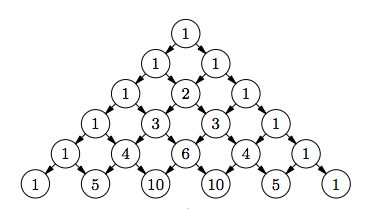
\includegraphics{Pascal_triangle}

\subsubsection{Упражнения}
1. $ A=\{1,2,3\} \quad B=\{2,3,4,5\} \quad A\cup B ? $\\
2. $ A = \{x \in N: \quad 2 < x < 4\} \quad B = \{x \in N: \quad 2 < x < 4\} \quad C = \{x \in N: \quad 2 < x < 4\} \quad B\cup C ?, A\cap B\cap C,A\cup B\cup C \quad ?$\\
3. $ (A\cap B)\cup C = (A\cup C)\cap(B\cup C)? $\\
4. $ (A \setminus B)\cap C = (A\cap C)\setminus (B\cap C) $\\
5. $ \left( 1-x\right)^5 = ?\\$
6. $ \left(\frac{2}{x} + 3 \sqrt[]{x} \right)^4 $\\
\section{Глава 2. Предел и непрерывность.}
\begin{mdframed}[backgroundcolor=blue!20] 
       Курс: Мат анализ (фтф:ИВТ)\\
       код слово: предел
    \end{mdframed}
\subsection{Параграф 1. Предел псоледовательности}
Предел -- пусть каждому натуральному числу N по некоторому закону поставленно в соответствие действительное число $ x_n $ тогда говорят что определена числовая последовательность $ \{x\} = \{x_1,x_2,....,x_n,...\} $ \\
Число a называется пределом последовательности $ \{x_n\}  $ если для всякого действительного числа $ \epsilon  > 0$ найдется зависящее от $ \epsilon $ число такое что выполняется неравенство $ |x_n - a| < \epsilon  $ для всех натуральных чисел $ n > n_0 $.  \\
\\Обозначение:\\
\[
	\lim_{n\to 0} x_n  = a \quad(x_n \to a \quad n \to \inf)	
\]
 
 \[
 	\lim_{n\to 0} x_n = a \Leftrightarrow  \quad \forall \epsilon > 0 \quad \exists n_0 = n_0(\epsilon): \forall n > n_0 \quad |x_n -a| < \epsilon
 \]
\begin{mdframed}[backgroundcolor=blue!20] 
       Пример: $  \lim_{n\to 0} \frac{1}{n}=0 $\\
       $|\frac{1}{n}| < \epsilon \quad \frac{1}{n} < \epsilon \quad n > \frac{1}{\epsilon} \quad n_0 = \left[\frac{1}{\epsilon}\right] + 1 \quad \forall \epsilon>0 $\\
       чтд.
    \end{mdframed}
Произвольный интервал $ AB $ содержащий точку С называется окресностью это точки\\
\[
	\cup(C)	
\]

Эпсилон окресность:\\
\[
	\cup(\epsilon)	\quad {\cup_\epsilon}(\epsilon) = \cup_\epsilon(\epsilon) \setminus {c}
\]
Число(точка) а является пределом последовательности $ x_n $
если для любого эпсилон больше нуля найдется число $ n_0 $ такое что все точки $ x_n $ с индексами $  n > n_0$ попадут в $ \epsilon $окресность точки а. Вне любой окресности точки а имеется конечная или пустое множество точек $ x_n $.



\subsection*{Литература}
Кудрявцев А.Д Курс математического анализа\\
Фихтенгольц Г.М Основы математического анализа\\
Демидович Б.П Сборник задач и упражнений по математическому анализу\\

\end{document}